%%%%%%%%%%%%%%%%%%%%%%%%%%%%%%%%%%%%%%%%%
% Jacobs Landscape Poster
% LaTeX Template
% Version 1.1 (14/06/14)
%
% Created by:
% Computational Physics and Biophysics Group, Jacobs University
% https://teamwork.jacobs-university.de:8443/confluence/display/CoPandBiG/LaTeX+Poster
% 
% Further modified by:
% Nathaniel Johnston (nathaniel@njohnston.ca)
%
% This template has been downloaded from:
% http://www.LaTeXTemplates.com
%
% License:
% CC BY-NC-SA 3.0 (http://creativecommons.org/licenses/by-nc-sa/3.0/)
%
%%%%%%%%%%%%%%%%%%%%%%%%%%%%%%%%%%%%%%%%%

%----------------------------------------------------------------------------------------
%	PACKAGES AND OTHER DOCUMENT CONFIGURATIONS
%----------------------------------------------------------------------------------------

%\documentclass[final]{beamer}
\documentclass[final]{beamer}
%\usepackage[scale=1.5]{beamerposter} % Use the beamerposter package for laying out the poster
\usepackage[scale=1.4]{beamerposter} 
\usetheme{confposter} % Use the confposter theme supplied with this template
\usepackage{pstricks}
%\usepackage{auto-pst-pdf}
\usepackage{graphicx}

\setbeamercolor{block title}{fg=ngreen,bg=white} % Colors of the block titles
\setbeamercolor{block body}{fg=black,bg=white} % Colors of the body of blocks
\setbeamercolor{block alerted title}{fg=white,bg=dblue!70} % Colors of the highlighted block titles
\setbeamercolor{block alerted body}{fg=black,bg=dblue!10} % Colors of the body of highlighted blocks
% Many more colors are available for use in beamerthemeconfposter.sty

%-----------------------------------------------------------
% Define the column widths and overall poster size
% To set effective sepwid, onecolwid and twocolwid values, first choose how many columns you want and how much separation you want between columns
% In this template, the separation width chosen is 0.024 of the paper width and a 4-column layout
% onecolwid should therefore be (1-(# of columns+1)*sepwid)/# of columns e.g. (1-(4+1)*0.024)/4 = 0.22
% Set twocolwid to be (2*onecolwid)+sepwid = 0.464
% Set threecolwid to be (3*onecolwid)+2*sepwid = 0.708

\newlength{\sepwid}
\newlength{\onecolwid}
\newlength{\twocolwid}
\newlength{\threecolwid}
\setlength{\paperwidth}{150cm} % A0 width: 46.8in
\setlength{\paperheight}{120cm} % A0 height: 33.1in
\setlength{\sepwid}{0.024\paperwidth} % Separation width (white space) between columns
\setlength{\onecolwid}{0.22\paperwidth} % Width of one column
\setlength{\twocolwid}{0.464\paperwidth} % Width of two columns
\setlength{\threecolwid}{0.708\paperwidth} % Width of three columns
\setlength{\topmargin}{-0.5in} % Reduce the top margin size
%-----------------------------------------------------------

%\usepackage{graphicx}  % Required for including images

\usepackage{booktabs} % Top and bottom rules for tables

%----------------------------------------------------------------------------------------
%	TITLE SECTION 
%----------------------------------------------------------------------------------------

\title{RNN-BASED MUSIC LANGUAGE MODELS FOR IMPROVING AUTOMATIC MUSIC TRANSCRIPTION} % Poster title

\author{Siddharth Sigtia$^\ast$,Emmanouil Benetos$^\dag$,Srikanth Cherla$^\dag$,Arter d'Avila Garcez$^\dag$,Tillman Weyde$^\dag$ and Simon Dixon$^\ast$} % Author(s)

\institute{$^\ast$ Centre for Digital Music, Queen Mary University of London\\
		   $^\dag$ Music Informatics Research Group, City University London\\ \vspace{0.2in}
		   \small{Contact: \texttt{s.s.sigtia@qmul.ac.uk}}} % Institution(s)

%----------------------------------------------------------------------------------------

\begin{document}

\addtobeamertemplate{block end}{}{\vspace*{2ex}} % White space under blocks
\addtobeamertemplate{block alerted end}{}{\vspace*{2ex}} % White space under highlighted (alert) blocks

\setlength{\belowcaptionskip}{2ex} % White space under figures
\setlength\belowdisplayshortskip{2ex} % White space under equations

\begin{frame}[t] % The whole poster is enclosed in one beamer frame

\begin{columns}[t] % The whole poster consists of three major columns, the second of which is split into two columns twice - the [t] option aligns each column's content to the top

\begin{column}{\sepwid}\end{column} % Empty spacer column

\begin{column}{\onecolwid} % The first column

%----------------------------------------------------------------------------------------
%	OBJECTIVES
%----------------------------------------------------------------------------------------

% \begin{alertblock}{Objectives}

% Lorem ipsum dolor sit amet, consectetur, nunc tellus pulvinar tortor, commodo eleifend risus arcu sed odio:
% \begin{itemize}
% \item Mollis dignissim, magna augue tincidunt dolor, interdum vestibulum urna
% \item Sed aliquet luctus lectus, eget aliquet leo ullamcorper consequat. Vivamus eros sem, iaculis ut euismod non, sollicitudin vel orci.
% \item Nascetur ridiculus mus.  
% \item Euismod non erat. Nam ultricies pellentesque nunc, ultrices volutpat nisl ultrices a.
% \end{itemize}

% \end{alertblock}

%----------------------------------------------------------------------------------------
%	INTRODUCTION
%----------------------------------------------------------------------------------------

\begin{block}{Introduction}

%In this paper, we investigate the use of Music Language Models (MLMs) for improving Automatic Music Transcription performance. The MLMs are trained on sequences of symbolic polyphonic music from the Nottingham dataset. We train Recurrent Neural Network (RNN)-based models, as they are capable of capturing complex temporal structure present in symbolic music data. Similar to the function of language models in automatic speech recognition, we use the MLMs to generate a prior probability for the occurrence of a sequence. The acoustic AMT model is based on probabilistic latent component analysis, and prior information from the MLM is incorporated into the transcription framework using Dirichlet priors. We test our hybrid models on a dataset of multiple-instrument polyphonic music and report a significant 3\% improvement in terms of F-measure, when compared to using an acoustic-only model.
\begin{itemize}
\item We investigate the problem of incorporating \textbf{symbolic} priors into automatic music transcription (AMT) systems.
%\item Traditional AMT algorithms model the acoustic signal but ignore higher level information present in the structure and patterns that appear in sequences of polyphonic music.
%\item Sequences of polyphonic music are comprised of repeating patterns and structures. Transcription systems can be 
\item An accurate model of higher-level symbolic music can potentially help improve transcription by providing a measure of expectations of predicted notes. 
\item Training accurate statistical models for predicting musical score is a harder problem than language modeling for speech. 
\item It is not immediately obvious how to combine the two sources of information together into a transcription system. 
\item We investigate one possible architecture using a recurrent neural network (RNN) \textbf{music language model} (MLM) and a spectrogram factorisatoin based acoustic model. 
\item The proposed architecture results in a $3\%$ improvement in F-measure on the Bach-10 dataset. 
\end{itemize}

\end{block}

%------------------------------------------------


\begin{block}{Language Modeling}

\begin{figure}
\centering
%\includegraphics[width=0.8\linewidth]{RNN.png}
\resizebox{800pt}{!}{% Generated with LaTeXDraw 2.0.8
% Mon Oct 13 12:03:09 BST 2014
% \usepackage[usenames,dvipsnames]{pstricks}
% \usepackage{epsfig}
% \usepackage{pst-grad} % For gradients
% \usepackage{pst-plot} % For axes
\scalebox{1} % Change this value to rescale the drawing.
{
\begin{pspicture}(0,-3.06)(24.98,3.06)
\psframe[linewidth=0.04,dimen=outer](4.6,3.06)(0.0,0.88)
\psframe[linewidth=0.04,dimen=outer](11.4,3.06)(6.8,0.88)
\psframe[linewidth=0.04,dimen=outer](18.16,3.06)(13.56,0.88)
\psframe[linewidth=0.04,linestyle=dashed,dash=0.16cm 0.16cm,dimen=outer](24.98,3.06)(20.38,0.88)
\psframe[linewidth=0.04,dimen=outer](4.6,-0.88)(0.0,-3.06)
\psframe[linewidth=0.04,dimen=outer](11.4,-0.88)(6.8,-3.06)
\psframe[linewidth=0.04,dimen=outer](18.16,-0.88)(13.56,-3.06)
\psline[linewidth=0.04cm,arrowsize=0.093cm 4.0,arrowlength=1.4,arrowinset=0.4]{->}(4.6,-2.0)(6.82,-2.0)
\psline[linewidth=0.04cm,arrowsize=0.093cm 4.0,arrowlength=1.4,arrowinset=0.4]{->}(11.42,-2.02)(13.62,-2.02)
\psline[linewidth=0.04cm,arrowsize=0.093cm 4.0,arrowlength=1.4,arrowinset=0.4]{->}(4.6,2.0)(6.82,2.0)
\psline[linewidth=0.04cm,arrowsize=0.093cm 4.0,arrowlength=1.4,arrowinset=0.4]{->}(11.38,2.0)(13.6,2.0)
\psline[linewidth=0.04cm,linestyle=dashed,dash=0.16cm 0.16cm,arrowsize=0.093cm 4.0,arrowlength=1.4,arrowinset=0.4]{->}(18.16,2.0)(20.38,2.0)
\psline[linewidth=0.04cm,linestyle=dashed,dash=0.16cm 0.16cm,arrowsize=0.093cm 4.0,arrowlength=1.4,arrowinset=0.4]{->}(18.14,-0.92)(20.34,0.9)
\psline[linewidth=0.04cm,arrowsize=0.093cm 4.0,arrowlength=1.4,arrowinset=0.4]{->}(11.4,-0.86)(13.6,0.96)
\psline[linewidth=0.04cm,arrowsize=0.093cm 4.0,arrowlength=1.4,arrowinset=0.4]{->}(4.62,-0.86)(6.82,0.96)
\psline[linewidth=0.04cm,arrowsize=0.093cm 4.0,arrowlength=1.4,arrowinset=0.4]{->}(2.26,0.86)(2.28,-0.92)
\psline[linewidth=0.04cm,arrowsize=0.093cm 4.0,arrowlength=1.4,arrowinset=0.4]{->}(9.12,0.88)(9.14,-0.9)
\psline[linewidth=0.04cm,arrowsize=0.093cm 4.0,arrowlength=1.4,arrowinset=0.4]{->}(15.88,0.86)(15.9,-0.92)
\usefont{T1}{ptm}{m}{n}
\rput(2.2628126,1.97){\large h(0)}
\usefont{T1}{ptm}{m}{n}
\rput(2.24125,-2.05){\large x(0)}
\usefont{T1}{ptm}{m}{n}
\rput(9.102813,2.05){\large h(1)}
\usefont{T1}{ptm}{m}{n}
\rput(9.08125,-2.03){\large x(1)}
\usefont{T1}{ptm}{m}{n}
\rput(15.90125,-1.97){\large x(2)}
\usefont{T1}{ptm}{m}{n}
\rput(15.842813,2.07){\large h(2)}
\usefont{T1}{ptm}{m}{n}
\rput(22.679375,2.085){...}
\end{pspicture} 
}

}
\caption{Generative RNN architecture}
\end{figure}
\begin{itemize}
%\item Polyphonic music prediction cannot be achieved with simple models such as n-grams which are popular in speech. 
\item RNNs are powerful models for polyphonic music prediction systems \cite{boulanger2012modeling}. 
%\item Hidden state summarizes the entire sequence. 
%\item Theoretically capable of learning dependencies between inputs over arbitrary lengths of time. 
\item One limitation is that the outputs of an RNN define unimodal distributions over output variables. 
%\item The RNN architecture is such that the output variables of the conditional distributions are independent of each other. 
\item This assumption of independence is violated by polyphonic music. 
\end{itemize}
\begin{figure}
\resizebox{800pt}{!}{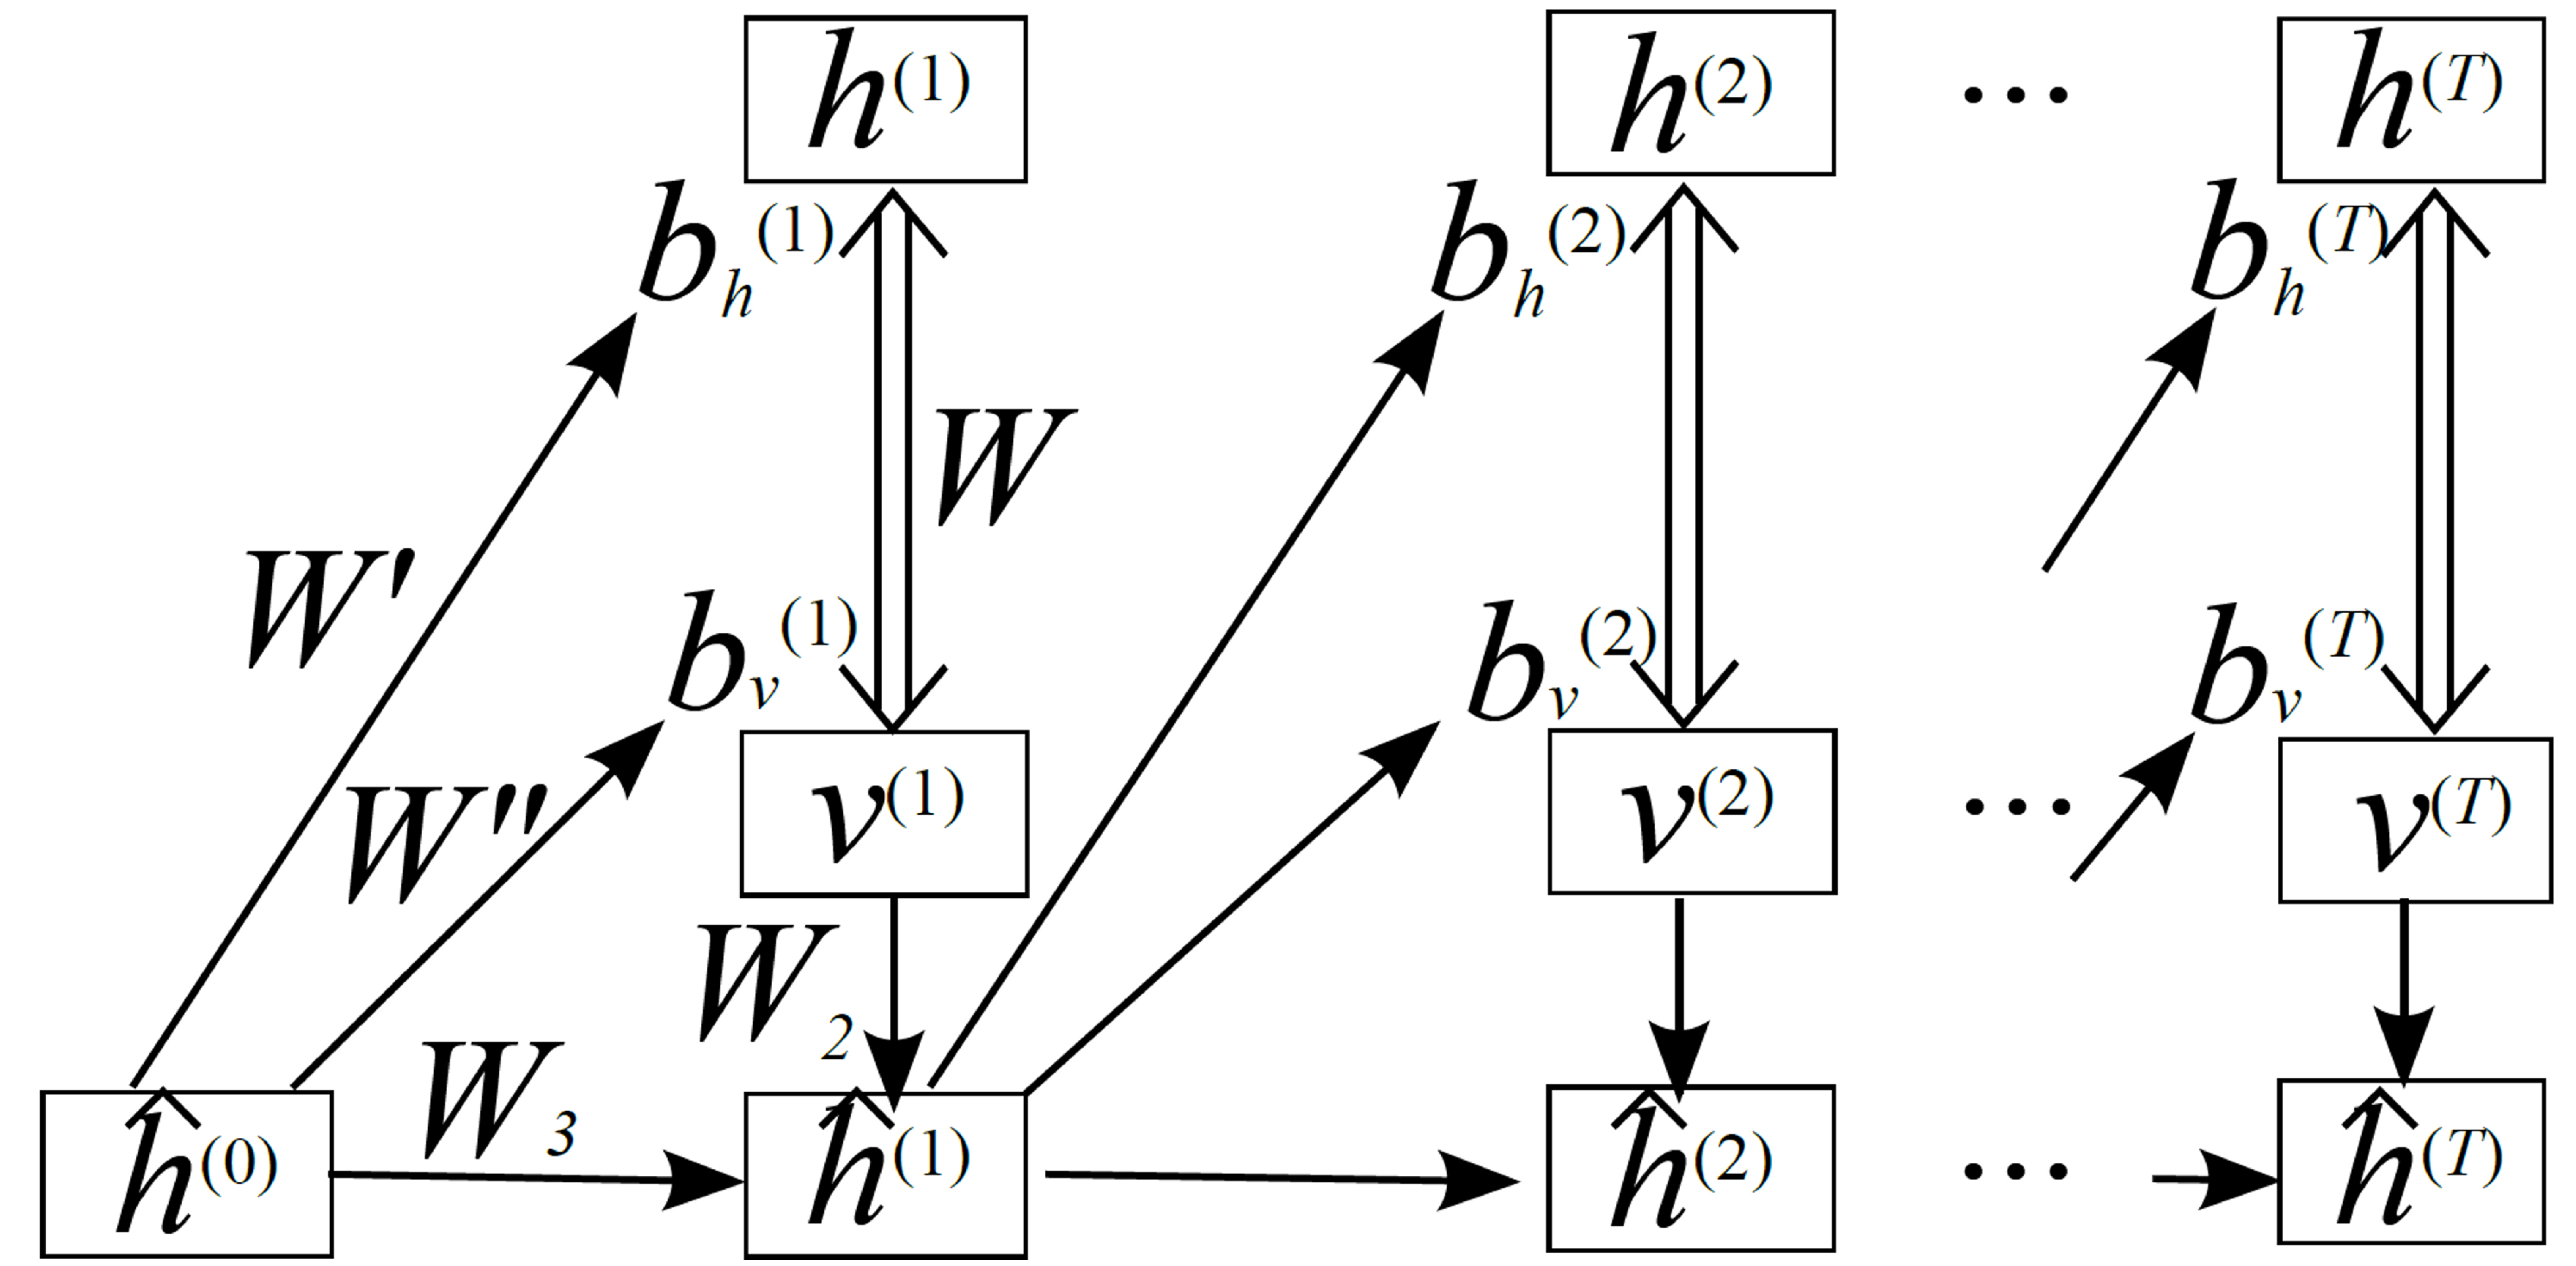
\includegraphics{outfile.eps}}
\caption{RNN-NADE architecture}
\end{figure}
\begin{itemize}
\item Multimodal conditional distributions can be modeled by allowing the RNN to predict parameters of a high-dimensional density estimator like the RBM or NADE. 
\item We use the NADE because calculating probabilities is tractable and it can be trained with Hessian Free (HF) optimisation. 
\end{itemize}
\end{block}


%----------------------------------------------------------------------------------------

\end{column} % End of the first column

\begin{column}{\sepwid}\end{column} % Empty spacer column

\begin{column}{\twocolwid} % Begin a column which is two columns wide (column 2)

\begin{columns}[t,totalwidth=\twocolwid] % Split up the two columns wide column

\begin{column}{\onecolwid}\vspace{-.6in} % The first column within column 2 (column 2.1)

%----------------------------------------------------------------------------------------
%	MATERIALS
%----------------------------------------------------------------------------------------

\begin{block}{Acoustic Modeling}

\begin{itemize}
\item We utilise the multiple-instrument transcription system based on probabilistic latent component analysis (PLCA). 
\item The input spectrogram $V_{\omega,t}$ is approximated as $P(\omega,t)$ ($\omega$: frequency, $t$: time). 
\end{itemize}
\setbeamercolor{block alerted title}{fg=black,bg=yellow} % Change the alert block title colors
\setbeamercolor{block alerted body}{fg=black,bg=white} % Change the alert block body colors

\begin{alertblock}{PLCA Model}

\begin{equation}
P(\omega,t) = P(t)\sum_{p,f,s}P(\omega|s,p,f)P_{t}(f|p)P_{t}(s|p)P_{t}(p) \label{eq:Model} \nonumber
\end{equation} 
\\
$P(t)$: Signal energy (known quantity). \\
$P(\omega|s,p,f)$: template for instrument $s$, pitch $p$, log-frequency shifting $f$. \\
$P_{t}(f|p)$: Time dependent pitch shifting (semitone range). 
$P_{t}(s|p)$: Time dependent source contribution per pitch.
$P_{t}(p)$: Pitch activation probability of $p$ at $t$. 
\end{alertblock}

\begin{itemize}
\item The unknown model parameters are estimated using the Expectation-Maximisation (EM) algorithm.
\item Using fixed sound templates $P(\omega|s,p,f)$, 20-30 iterations of the EM algorithm are sufficient for convergence. 
\end{itemize}

\end{block}

\begin{block}{Proposed Transcription System}
\begin{figure}
\includegraphics[width=0.9\linewidth]{FigSystem.eps}
\caption{Proposed Transcription Architecture}
\end{figure}

%----------------------------------------------------------------------------------------
\begin{itemize}
\item The outputs of the PLCA acoustic model form a multinomial distribution. 
\item The Dirichlet distribution is conjugate to the multinomial distribution and a Dirichlet prior can be used to combine the two sources of information.
\item Dirichlet prior for pitch activation: $\alpha_t(p) = P_t(p)P_{MLM}(p,t)$
\item The recording is re-transcribed using the following equation.
\begin{equation}
 P_{t}(p) \propto \sum_{\omega,f,s}P_{t}(p,f,s|\omega)V_{\omega,t}+\kappa\alpha_{t}(p) \label{eq:modifiedMStepPitchActivation} 
\end{equation}
\item $\kappa$ is a parameter that controls the degree of influence of the prior. $\kappa$ is decressed from 1 to 0 over subsequent iterations.
\item Therefore, the transcription yields a symbolic prediction, which improves the subsequent re-transcription of the input. 
\end{itemize}
\end{block}
\end{column} % End of column 2.1

\begin{column}{\onecolwid}\vspace{-.6in} % The second column within column 2 (column 2.2)

%----------------------------------------------------------------------------------------
%	METHODS
%----------------------------------------------------------------------------------------

\begin{block}{Validation}

\begin{table}[t]
 \begin{center}
 \scalebox{1.}{
 \begin{tabular}{|l|c|}
  \hline
  \textbf{Model} & $\mathit{Pre}$ \\ \hline 
  RNN (SGD)  & 67.89\% \\ \hline
  RNN (HF) & 69.61\% \\ \hline
  RNN-NADE (SGD) & 68.89\% \\ \hline
  RNN-NADE (HF)  & \textbf{70.61}\% \\ \hline
 \end{tabular}
 }
\end{center} 
\caption{Validation results for MLMs}
\end{table}

\begin{itemize}
\item The language models are trained on the Nottingham dataset, a collection of 1200 folk melodies. 
\item We evaluate the performance of the RNN and the RNN-NADE models on a music prediction task for validation. 
\item Both models are trained in 2 different ways; Stochastic Gradient Descent (SGD) and Hessian Free (HF) Optimisation.
\item Table 1 enumerates the expected precision for a music prediction task. 
\end{itemize}
\end{block}

%----------------------------------------------------------------------------------------

\begin{block}{Results}

\begin{table}[t]
 \begin{center}
 \scalebox{1}{
 \begin{tabular}{|l|c|c|c|}
  \hline
  \textbf{Configuration} & $\mathit{F}$ & $\mathit{Pre}$ & $\mathit{Rec}$  \\ \hline 
  Configuration 1 & 62.02\%  & 58.51\% & 66.12\% \\ \hline
  Configuration 2 - NADE & 62.62\% & 59.70\% & 65.92\% \\ \hline
  Configuration 3 - NADE & 64.08\% & 61.96\% & 66.44\% \\ \hline
  Configuration 2 - RNN & 62.29\% & 59.08\% & 65.98\% \\ \hline
  Configuration 3 - RNN & 63.85\% & 61.14\% & 66.90\% \\ \hline  
  Configuration 2 - NADE-HF & 62.20\% & 59.14\% & 65.68\% \\ \hline
  Configuration 3 - NADE-HF & \textbf{65.16}\% & \textbf{62.80}\% & \textbf{67.78}\% \\ \hline  
  Configuration 2 - RNN-HF & 62.44\% & 59.28\% & 66.07\% \\ \hline
  Configuration 3 - RNN-HF & 62.87\% & 60.03\% & 66.11\% \\ \hline    
 \end{tabular}
 }
\end{center}
 \caption{Transcription results using various system configurations.}
 \label{tab:results}
\end{table}

\begin{itemize}
\item Transcription experiments are performed on the Bach-10 dataset, a multi-track collection of multiple-instrument polyphonic music.
\item We evaluate three different configurations for transcription experiments
\end{itemize}

\setbeamercolor{block alerted title}{fg=black,bg=yellow} % Change the alert block title colors
\setbeamercolor{block alerted body}{fg=black,bg=white} % Change the alert block body colors
\begin{alertblock}{Configurations}
\begin{itemize}
\item Configuration 1: PLCA Acoustic model only. \\
\item Configuration 2: Predictions from acoustic model as inputs to MLM. 
\item Configuration 3: MLM used to re-transcribe recordings according to Equation 1.
\end{itemize}
\end{alertblock}
\begin{itemize}
 \item Results from table 2 demonstrate that the MLM can be trained on data from a different source as compared to the acoustic model.
\end{itemize}

%\begin{itemize}
%\item Table 2 summarizes the results of the transcription experiments on the Bach-10 dataset using the different configurations.
%\end{itemize}

\end{block}



\end{column} % End of column 2.2

\end{columns} % End of the split of column 2 - any content after this will now take up 2 columns width

%----------------------------------------------------------------------------------------
%	IMPORTANT RESULT
%----------------------------------------------------------------------------------------

% \begin{alertblock}{Important Result}

% Lorem ipsum dolor \textbf{sit amet}, consectetur adipiscing elit. Sed commodo molestie porta. Sed ultrices scelerisque sapien ac commodo. Donec ut volutpat elit.

% \end{alertblock} 

%----------------------------------------------------------------------------------------

% \begin{columns}[t,totalwidth=\twocolwid] % Split up the two columns wide column again

% \begin{column}{\onecolwid} % The first column within column 2 (column 2.1)

% %----------------------------------------------------------------------------------------
% %	MATHEMATICAL SECTION
% %----------------------------------------------------------------------------------------

% \begin{block}{Mathematical Section}

% Nam quis odio enim, in molestie libero. Vivamus cursus mi at nulla elementum sollicitudin. Nam quis odio enim, in molestie libero. Vivamus cursus mi at nulla elementum sollicitudin.
  
% \begin{equation}
% E = mc^{2}
% \label{eqn:Einstein}
% \end{equation}

% Nam quis odio enim, in molestie libero. Vivamus cursus mi at nulla elementum sollicitudin. Nam quis odio enim, in molestie libero. Vivamus cursus mi at nulla elementum sollicitudin.

% \begin{equation}
% \cos^3 \theta =\frac{1}{4}\cos\theta+\frac{3}{4}\cos 3\theta
% \label{eq:refname}
% \end{equation}

% Nam quis odio enim, in molestie libero. Vivamus cursus mi at nulla elementum sollicitudin. Nam quis odio enim, in molestie libero. Vivamus cursus mi at nulla elementum sollicitudin.

% \begin{equation}
% \kappa =\frac{\xi}{E_{\mathrm{max}}} %\mathbb{ZNR}
% \end{equation}

% \end{block}

% %----------------------------------------------------------------------------------------

% \end{column} % End of column 2.1

% \begin{column}{\onecolwid} % The second column within column 2 (column 2.2)

% %----------------------------------------------------------------------------------------
% %	RESULTS
% %----------------------------------------------------------------------------------------

% \begin{block}{Results}

% \begin{figure}
% \includegraphics[width=0.8\linewidth]{placeholder.jpg}
% \caption{Figure caption}
% \end{figure}

% Nunc tempus venenatis facilisis. Curabitur suscipit consequat eros non porttitor. Sed a massa dolor, id ornare enim:

% \begin{table}
% \vspace{2ex}
% \begin{tabular}{l l l}
% \toprule
% \textbf{Treatments} & \textbf{Response 1} & \textbf{Response 2}\\
% \midrule
% Treatment 1 & 0.0003262 & 0.562 \\
% Treatment 2 & 0.0015681 & 0.910 \\
% Treatment 3 & 0.0009271 & 0.296 \\
% \bottomrule
% \end{tabular}
% \caption{Table caption}
% \end{table}

% \end{block}

% %----------------------------------------------------------------------------------------

% \end{column} % End of column 2.2

% \end{columns} % End of the split of column 2

\end{column} % End of the second column

\begin{column}{\sepwid}\end{column} % Empty spacer column

\begin{column}{\onecolwid} % The third column

%----------------------------------------------------------------------------------------
%	CONCLUSION
%----------------------------------------------------------------------------------------

\begin{block}{Discussion}

\begin{itemize}
\item From table 2, we observe the RNN-NADE MLM performs best when used in configuration 3.
\item When using the MLMs to provide priors for re-transcription, the F-measure improves by $3\%$ over an acoustic only transcription configuration.
\item Training the MLMs with HF appears to help improve transcription results.
\end{itemize}

\begin{figure}
\includegraphics[width=0.9\linewidth]{FigSpectrogram.eps}
\caption{(a) The spectrogram $V_{\omega,t}$ for a recording. (b) The pitch activation $P(p,t)$ using the  transcription-prediction system with the NADE-HF.}
\end{figure}

\begin{figure}
\includegraphics[width=0.9\linewidth]{FigTranscription.eps}
\caption{(a) Post-processed output of the transcription-prediction system with the NADE-HF. (b) The pitch ground truth of the recording.}
\end{figure}

\end{block}

%----------------------------------------------------------------------------------------
%	ADDITIONAL INFORMATION
%----------------------------------------------------------------------------------------

%----------------------------------------------------------------------------------------
%	REFERENCES
%----------------------------------------------------------------------------------------

\begin{block}{References}

\nocite{*} % Insert publications even if they are not cited in the poster
\small{\bibliographystyle{unsrt}
\bibliography{sample}\vspace{0.75in}}

\end{block}

%----------------------------------------------------------------------------------------
%	ACKNOWLEDGEMENTS
%---------------------------------------------------------------------------------------- % Change the block title color



\end{column} % End of the third column

\end{columns} % End of all the columns in the poster

\end{frame} % End of the enclosing frame

\end{document}
